\chapter{図形を描く}
\label{chap:drawing-shapes}

この章では、p5.jsを使って点、線、円、長方形、三角形、四角形を描く方法を学びます。座標を使って図形の位置を決め、命令を並べる順番によって重なり方を考えながら、TypeScript + p5.js instance modeで図形を描いていきます。

\section{この章の概要}

コンピュータで絵を描くときには、「どこに」「どのような大きさで」描くかを数値で指定します。最初は数値が多く見えるかもしれませんが、どの数値が位置を表し、どの数値が大きさを表すのかを分けて考えると読みやすくなります。

この章で扱う主な内容は次の通りです。

\begin{itemize}
    \item サンプルを読むためのJavaScriptの短い復習
    \item キャンバスと座標の考え方
    \item 点と線の描き方
    \item 円、楕円、長方形の描き方
    \item 三角形と四角形の描き方
    \item 描く順番による見え方の違い
    \item 複数の図形を組み合わせる考え方
\end{itemize}

\section{JavaScriptの書き方を復習する}

第1章で動かしたスケッチには、JavaScriptやTypeScriptの記号がいくつか使われていました。以前にJavaScriptを学んだことがあっても、記号の意味をすぐに思い出せないことがあります。この節では、これからサンプルを読むために必要な部分だけを短く復習します。すべてを暗記する必要はなく、分からなくなったときにここへ戻って確認できれば十分です。

まず、サンプルでよく使う記号とインデントの読み方を確認します。

\begin{table}[H]
    \centering
    \caption{サンプルを読むために使う記号}
    \label{tab:chapter02-javascript-symbols}
    \begin{tabular}{p{0.13\linewidth}p{0.31\linewidth}p{0.46\linewidth}}
        \toprule
        記号 & 呼び方・使う場所 & 読み方 \\
        \midrule
        \texttt{\{ \}}
            & 波括弧
            & 関数などに含まれる処理の始まりと終わりを表します。対応する開き括弧と閉じ括弧を探します。 \\
        \texttt{( )}
            & 丸括弧
            & 関数を定義するときは受け取る値の名前を、呼び出すときは渡す値を書きます。\texttt{()}は、それらがないことを表します。 \\
        \texttt{;}
            & セミコロン
            & 1つの文の終わりを表します。本書のサンプルでは、文の最後に付けます。 \\
        インデント
            & 行の先頭の空白
            & どの処理が\texttt{\{ \}}の内側にあるかを見やすくします。同じ深さの行は、先頭をそろえます。 \\
        \bottomrule
    \end{tabular}
\end{table}

\texttt{p.circle(200, 150, 80);}のように、関数の名前の後ろへ丸括弧を書いたものは、\textbf{関数呼び出し}です。丸括弧の中に書く\texttt{200}、\texttt{150}、\texttt{80}のような値を\textbf{引数}と呼びます。この例では、\texttt{p.circle}関数へ、円の中心のx座標、中心のy座標、直径を順番に渡しています。

引数はコンマで区切り、関数ごとに個数と順番が決まっています。たとえば、\texttt{p.createCanvas(400, 300)}では、最初の引数がキャンバスの幅、次の引数が高さです。引数の詳しい考え方は、第8章「関数で整理する」で扱います。

値に名前を付けるときには、\texttt{const}または\texttt{let}を使います。途中で値を変えない場合は\texttt{const}、あとで値を変える場合は\texttt{let}を使います。

\begin{center}
\begin{tabular}{lll}
    \toprule
    書き方 & 意味 & 例 \\
    \midrule
    \texttt{const} & あとから別の値を代入しない & \texttt{const diameter: number = 80;} \\
    \texttt{let} & あとから値を変えることができる & \texttt{let circleX: number = 100;} \\
    \bottomrule
\end{tabular}
\end{center}

ここでは、サンプルの中で\texttt{const}と\texttt{let}を見分けられれば十分です。変数、型注釈、\texttt{const}と\texttt{let}の使い分けは、第4章「変数と型注釈」で詳しく説明します。

JavaScriptとTypeScriptでは、\texttt{=}と\texttt{===}の意味が異なります。

\begin{center}
\begin{tabular}{lll}
    \toprule
    記号 & 意味 & 例 \\
    \midrule
    \texttt{=} & 右側の値や処理を左側へ代入する & \texttt{circleX = 200;} \\
    \texttt{===} & 左右の値が等しいか比較する & \texttt{circleX === 200} \\
    \bottomrule
\end{tabular}
\end{center}

\texttt{circleX = 200;}は、\texttt{circleX}へ\texttt{200}を代入する文です。一方、\texttt{circleX === 200}は、値が等しければ\texttt{true}、等しくなければ\texttt{false}になる比較です。比較は、第6章「条件分岐とインタラクション」で詳しく扱います。

\texttt{//}から行の終わりまでは\textbf{コメント}です。コメントはプログラムの説明として人が読むためのもので、処理としては実行されません。本書では、変数が何を表すか、なぜその処理が必要かを示すためにコメントを使います。

プログラムに間違いがあると、VS Codeに赤い波線が表示されたり、ターミナルやブラウザにエラーメッセージが表示されたりします。最初から英語のメッセージをすべて理解する必要はありません。まず、ファイル名と行番号を探し、その行の括弧、セミコロン、関数名、引数の個数を確認しましょう。VS Codeの赤い波線へマウスポインタを重ねると、間違いの手掛かりが表示されます。

\begin{pointbox}{エラーは修正場所を探す手掛かり}
エラーメッセージは、失敗を知らせるだけのものではなく、どこを確認すればよいかを示す手掛かりです。最初に表示されたエラーのファイル名と行番号から確認し、修正したらもう一度保存して動作を確かめましょう。
\end{pointbox}

\section{キャンバスと座標}

p5.jsでは、図形を描くための領域をキャンバス\footnote{英語では、canvasと書きます。}と呼びます。
instance modeでは、スケッチを表す\texttt{p}を通して\texttt{p.createCanvas}を呼び出し、キャンバスを作ります。
\texttt{p.createCanvas(400, 300)}は、幅400、高さ300のキャンバスを作る命令です。

\begin{listing}[htbp]
\begin{minted}{ts}
p.createCanvas(400, 300);
\end{minted}
\caption{幅400、高さ300のキャンバスを作る}
\label{lst:chapter02-create-canvas}
\end{listing}

この例では、横400ピクセル、縦300ピクセルのキャンバスを作っています。ピクセル\footnote{英語では、pixelと書きます。日本語では画素と呼ぶこともあります。}とは、画面上の小さな点のことです。デジタル画像は、このピクセルの集まりとして表示されます。

\begin{figure}[htbp]
    \centering
    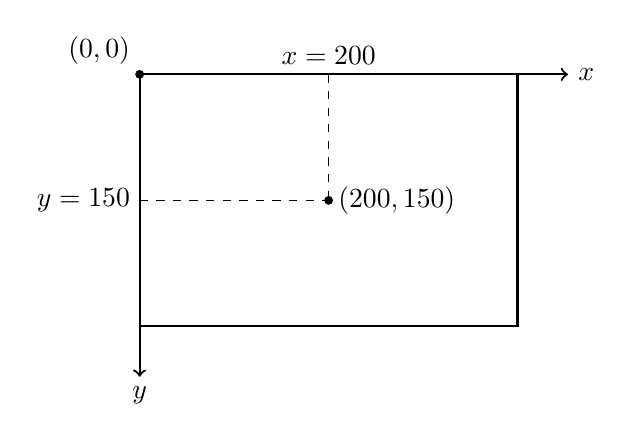
\begin{tikzpicture}[scale=0.8]
        \draw[thick] (0,0) rectangle (6,-4);    %%% ここを修正
        \draw[->,thick] (0,0) -- (6.8,0) node[right] {$x$};
        \draw[->,thick] (0,0) -- (0,-4.8) node[below] {$y$};
        \fill (0,0) circle (2pt);
        \node[above left] at (0,0) {$(0, 0)$};
        \fill (3,-2) circle (2pt);
        \node[right] at (3,-2) {$(200, 150)$};
        \draw[dashed] (3,0) -- (3,-2);
        \draw[dashed] (0,-2) -- (3,-2);
        \node[above] at (3,0) {$x=200$};
        \node[left] at (0,-2) {$y=150$};
    \end{tikzpicture}
    \caption{p5.jsの座標の考え方}
    \label{fig:chapter02-coordinate-system}
\end{figure}

画面上のピクセルの位置を表すために、高校まで数学で学んだグラフのように、水平方向に$X$軸、垂直方向に$Y$軸を考えます。
数学のグラフでは、右に進むほど $X$座標の値が大きくなり、上に進むほど $Y$座標の値が大きくなります。
一方、p5.jsなどのコンピュータの世界では、左上が原点で、下に進むほど $Y$座標の値が大きくなりますことが多いです（図\ref{fig:chapter02-coordinate-system}）。
この違いはとても重要です。

\section{点と線を描く}
\label{sec:points-and-lines}

点を描くには、その点の $X$ 座標と $Y$ 座標を指定します。
線を描くには、線分の始点と終点の $X$ 座標と $Y$ 座標を指定します。

\begin{listing}[htbp]
\inputminted{ts}{listings/chapter02/points-and-lines.ts}
\caption{点と線を描く}
\label{lst:chapter02-points-and-lines}
\end{listing}

9行目の\texttt{p.background(250)}は、キャンバスの背景を白に近い灰色で塗りつぶす命令です。
引数の数値は、0から255までの範囲で、0が黒、255が白のように明るさが変化します。
\texttt{p.point(80, 80)}は、$X$ 座標が80、$Y$ 座標が80の位置に点を描きます。\texttt{p.line(80, 80, 320, 220)}は、$(80, 80)$から$(320, 220)$までの線分を描きます。
また、点や線の太さを変えるには、\texttt{strokeWeight}関数を使います。
引数に指定した数値が大きいほど、点や線は太くなります。
例えば、11行目の\texttt{p.strokeWeight(8)}により点を見やすくし、その後、16行目の\texttt{p.strokeWeight(2)}で線を少し細くしてから線分を描いています。

8行目から17行目で指定された命令は、上から順に実行されます。
7行目から18行目では、最初に1回だけ実行される\texttt{setup}関数を定義していることになっています。

Javascriptの事をよく知っている人には、このサンプルの7行目から18行目は、JavaScriptのアロー関数を使った書き方で、
関数\texttt{setup}の定義を行っていると言った方が簡単に理解できるかもしれません。
同じように、5行目から19行目では、\texttt{sketch}関数の定義を行っています。

この節で使われた関数をまとめると、次の表のようになります。

\begin{table}[htbp]
\centering
\begin{tabular}{ll}
\toprule
関数 & 説明 \\
\midrule
\texttt{setup()} & 1回だけ実行される初期化用の関数、動作はプログラムが決める \\
\texttt{createCanvas(w, h)} & 幅$w$、高さ$h$のキャンバスを作る \\
\texttt{background(gray)} & キャンバスを灰色の明るさ$gray$で塗りつぶす \\
\texttt{point(x, y)} & 座標$(x, y)$に点を描く \\
\texttt{line(x1, y1, x2, y2)} & 座標$(x1, y1)$から$(x2, y2)$までの線分を描く \\
\texttt{strokeWeight(w)} & 線の太さや点の大きさを$w$にする \\
\bottomrule
\end{tabular}
\caption{節\ref{sec:points-and-lines}で使った関数}
\label{tab:chapter02-points-and-lines}
\end{table}

表\ref{tab:chapter02-points-and-lines}で紹介した\texttt{point}、\texttt{line}、\texttt{strokeWeight}は、図\ref{fig:chapter02-point-line-strokeweight}のような関係にあります。
\texttt{point}は1つの座標に点を置き、\texttt{line}は2つの座標を結びます。
\texttt{strokeWeight}は、その後に描く点や線の太さを変える命令です。

\begin{figure}[htbp]
    \centering
    \begin{tikzpicture}[x=1cm, y=1cm, font=\small]
        \tikzset{
            canvas/.style={draw=black!70, fill=gray!5, line width=0.6pt},
            guide/.style={draw=gray!35, dashed, line width=0.4pt},
            markpoint/.style={fill=black},
            labeltext/.style={font=\small\ttfamily}
        }

        \begin{scope}[shift={(0,0)}]
            \draw[canvas] (0,0) rectangle (3.5,-2.4);
            \draw[guide] (1.75,0) -- (1.75,-1.2);
            \draw[guide] (0,-1.2) -- (1.75,-1.2);
            \fill[markpoint] (1.75,-1.2) circle (2.2pt);
            \node[labeltext] at (1.75,-2.85) {point(x, y)};
            \node[align=center] at (1.75,-3.35) {指定した座標に\\点を描く};
        \end{scope}

        \begin{scope}[shift={(4.4,0)}]
            \draw[canvas] (0,0) rectangle (3.5,-2.4);
            \fill[markpoint] (0.7,-0.6) circle (1.8pt);
            \fill[markpoint] (2.8,-1.8) circle (1.8pt);
            \draw[line width=1.1pt] (0.7,-0.6) -- (2.8,-1.8);
            \node[above right, font=\scriptsize] at (0.7,-0.6) {$(x_1,y_1)$};
            \node[below left, font=\scriptsize] at (2.8,-1.8) {$(x_2,y_2)$};
            \node[labeltext] at (1.75,-2.85) {line(x1, y1, x2, y2)};
            \node[align=center] at (1.75,-3.35) {始点と終点を\\線で結ぶ};
        \end{scope}

        \begin{scope}[shift={(8.8,0)}]
            \draw[canvas] (0,0) rectangle (3.5,-2.4);
            \draw[line width=0.5pt] (0.45,-0.55) -- (1.45,-0.55);
            \draw[line width=2.6pt] (2.05,-0.55) -- (3.05,-0.55);
            \fill[markpoint] (0.95,-1.55) circle (1.2pt);
            \fill[markpoint] (2.55,-1.55) circle (4.5pt);
            \node[font=\scriptsize] at (0.95,-0.95) {$w=1$};
            \node[font=\scriptsize] at (2.55,-0.95) {$w=8$};
            \node[labeltext] at (1.75,-2.85) {strokeWeight(w)};
            \node[align=center] at (1.75,-3.35) {点や線の\\太さを変える};
        \end{scope}
    \end{tikzpicture}
    \caption{\texttt{point}、\texttt{line}、\texttt{strokeWeight}の働き}
    \label{fig:chapter02-point-line-strokeweight}
\end{figure}

\begin{notebox}{点が小さく見えるとき}
点はそのままだと小さく見えます。このサンプルでは、見やすくするために\texttt{p.strokeWeight(8)}で点や線の太さを変えています。線の太さや色の詳しい指定は、次の章で扱います。
\end{notebox}

\section{円、楕円、長方形を描く}

円や長方形も、位置と大きさを数値で指定して描きます。最初は、中心を指定する図形と、左上の位置を指定する図形の違いに注意しましょう。

\begin{listing}[htbp]
\inputminted{ts}{listings/chapter02/ellipses-and-rectangles.ts}
\caption{円、楕円、長方形を描く}
\label{lst:chapter02-ellipses-and-rectangles}
\end{listing}

\texttt{p.ellipse(120, 120, 160, 120)}は、中心が$(120, 120)$、幅が160、高さが120の楕円を描きます。\texttt{p.circle(300, 120, 100)}は、中心が$(300, 120)$、直径が100の円を描きます。

\texttt{p.rect(360, 70, 80, 100)}は、左上の位置が$(360, 70)$、幅が80、高さが100の長方形を描きます。円や楕円と長方形では、最初の2つの数値の意味が少し違います。

この節で使われた関数をまとめると、次の表のようになります。

\begin{table}[htbp]
\centering
\begin{tabular}{ll}
\toprule
関数 & 説明 \\
\midrule
\texttt{ellipse(x, y, w, h)} & 中心$(x, y)$、幅$w$、高さ$h$の楕円を描く \\
\texttt{circle(x, y, d)} & 中心$(x, y)$、直径$d$の円を描く \\
\texttt{rect(x, y, w, h)} & 左上の位置$(x, y)$、幅$w$、高さ$h$の長方形を描く \\
\bottomrule
\end{tabular}
\caption{円、楕円、長方形を描く関数}
\label{tab:chapter02-ellipses-and-rectangles}
\end{table}

表\ref{tab:chapter02-ellipses-and-rectangles}で紹介した3つの関数は、図\ref{fig:chapter02-ellipse-circle-rect}のような図形を描きます。
\texttt{ellipse}と\texttt{circle}は中心の位置を決めてから図形の大きさを指定します。
一方、\texttt{rect}は左上の位置を決めてから、右方向の幅と下方向の高さを指定します。

\begin{figure}[htbp]
    \centering
    \begin{tikzpicture}[x=0.95cm, y=0.95cm, font=\small]
        \tikzset{
            canvas/.style={draw=black!70, fill=gray!5, line width=0.6pt},
            guide/.style={draw=gray!40, dashed, line width=0.4pt},
            drawnshape/.style={draw=black, fill=gray!18, line width=1pt},
            basepoint/.style={fill=black},
            labeltext/.style={font=\small\ttfamily}
        }

        \begin{scope}[shift={(0,0)}]
            \draw[canvas] (0,0) rectangle (3.5,-2.6);
            \draw[drawnshape] (1.75,-1.25) ellipse (1.15 and 0.65);
            \draw[guide] (0.6,-1.25) -- (2.9,-1.25);
            \draw[guide] (1.75,-0.6) -- (1.75,-1.9);
            \fill[basepoint] (1.75,-1.25) circle (2pt);
            \node[above, font=\scriptsize] at (1.75,-1.25) {中心};
            \draw[<->, font=\scriptsize] (0.6,-2.15) -- node[below] {$w$} (2.9,-2.15);
            \draw[<->, font=\scriptsize] (3.1,-0.6) -- node[right] {$h$} (3.1,-1.9);
            \node[labeltext] at (1.75,-3.05) {ellipse(x, y, w, h)};
            \node[align=center] at (1.75,-3.55) {中心と幅・高さで\\楕円を描く};
        \end{scope}

        \begin{scope}[shift={(4.4,0)}]
            \draw[canvas] (0,0) rectangle (3.5,-2.6);
            \draw[drawnshape] (1.75,-1.25) circle (0.75);
            \draw[guide] (1.0,-1.25) -- (2.5,-1.25);
            \fill[basepoint] (1.75,-1.25) circle (2pt);
            \node[above, font=\scriptsize] at (1.75,-1.25) {中心};
            \draw[<->, font=\scriptsize] (1.0,-2.15) -- node[below] {$d$} (2.5,-2.15);
            \node[labeltext] at (1.75,-3.05) {circle(x, y, d)};
            \node[align=center] at (1.75,-3.55) {中心と直径で\\円を描く};
        \end{scope}

        \begin{scope}[shift={(8.8,0)}]
            \draw[canvas] (0,0) rectangle (3.5,-2.6);
            \draw[drawnshape] (0.85,-0.65) rectangle (2.75,-1.9);
            \fill[basepoint] (0.85,-0.65) circle (2pt);
            \node[above right, font=\scriptsize] at (0.85,-0.65) {左上};
            \draw[<->, font=\scriptsize] (0.85,-2.15) -- node[below] {$w$} (2.75,-2.15);
            \draw[<->, font=\scriptsize] (3.0,-0.65) -- node[right] {$h$} (3.0,-1.9);
            \node[labeltext] at (1.75,-3.05) {rect(x, y, w, h)};
            \node[align=center] at (1.75,-3.55) {左上と幅・高さで\\長方形を描く};
        \end{scope}
    \end{tikzpicture}
    \caption{\texttt{ellipse}、\texttt{circle}、\texttt{rect}で描かれる図形}
    \label{fig:chapter02-ellipse-circle-rect}
\end{figure}

\begin{pointbox}{中心で指定する図形と左上で指定する図形}
\texttt{ellipse}や\texttt{circle}は中心の座標を指定します。\texttt{rect}は基本的に左上の座標を指定します。どの点を基準にしているかを意識すると、図形を配置しやすくなります。
\end{pointbox}

\section{三角形と四角形を描く}

三角形や四角形は、頂点の座標を順番に指定して描きます。少し数値が多くなりますが、「1つの頂点に$x$と$y$の2つの数値が必要」と考えると整理しやすくなります。

\begin{listing}[htbp]
\inputminted{ts}{listings/chapter02/triangles-and-quads.ts}
\caption{三角形と四角形を描く}
\label{lst:chapter02-triangles-and-quads}
\end{listing}

\begin{figure}[http]
    \centering
    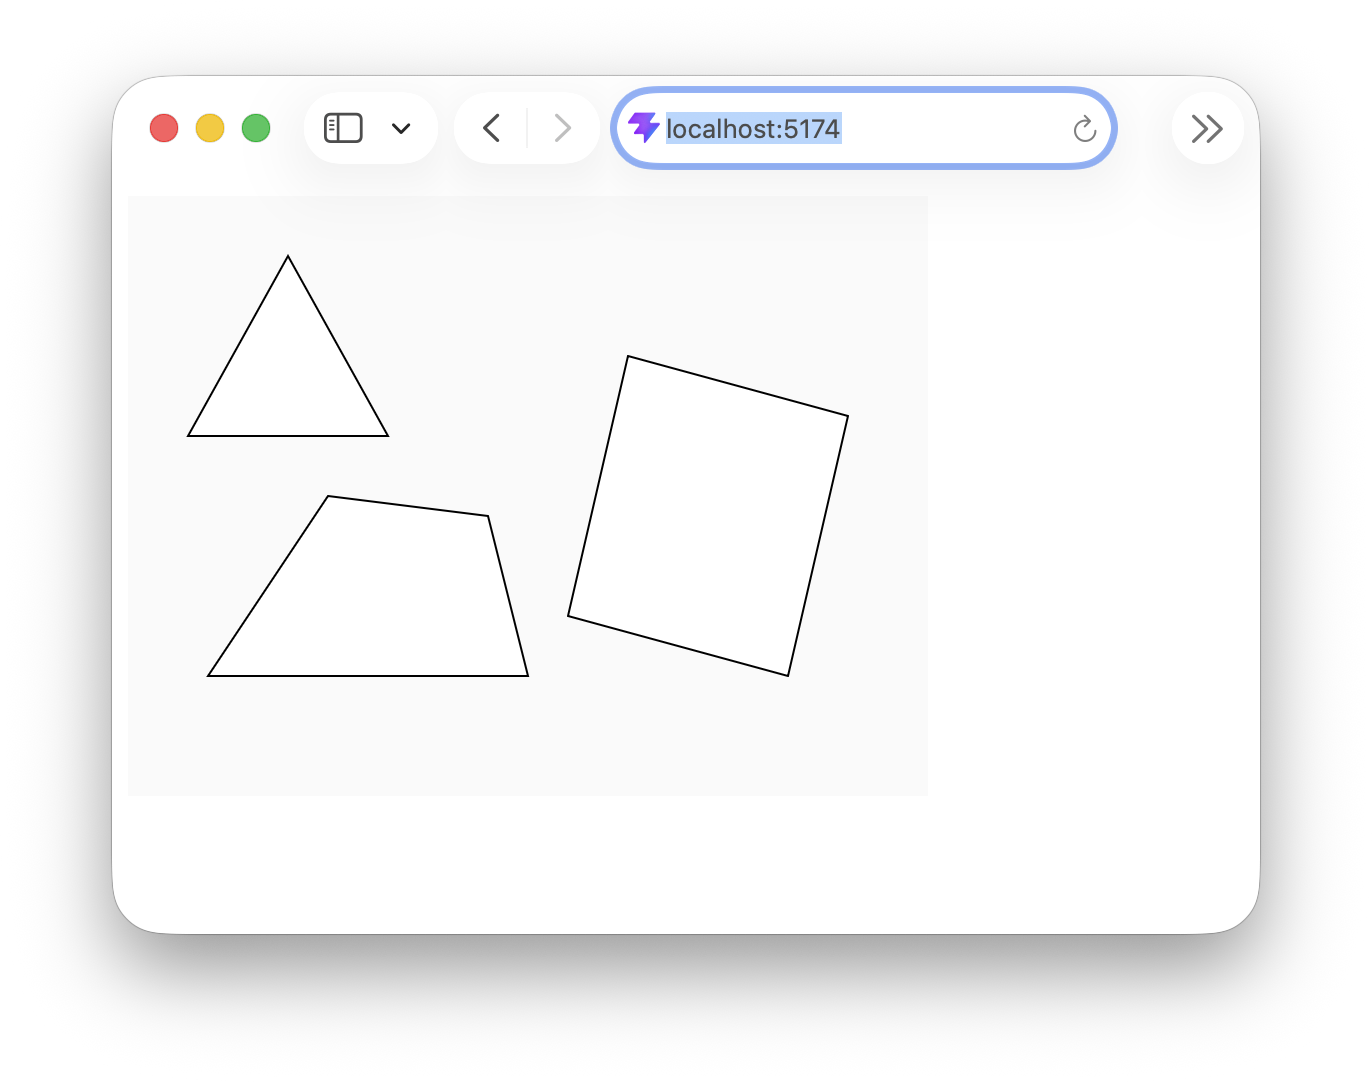
\includegraphics[width=0.6\linewidth]{figures/chapter02/triangle-quad.png}
    \caption{三角形と四角形の描画例}
    \label{fig:chapter02-triangle-quad}
\end{figure}

\texttt{triangle}関数では3つの頂点を指定します。つまり、合計で6つの数値を使います。
\texttt{quad}関数では4つの頂点を指定するため、合計で8つの数値を使います。
\texttt{rect}関数は、長方形（矩形）を描くための関数ですが、\texttt{quad}関数では、台形のような形も描くことができます。

\begin{table}[htbp]
\centering
\begin{tabular}{lp{0.52\linewidth}}
\toprule
関数 & 説明 \\
\midrule
\texttt{triangle(x1, y1, x2, y2,x3, y3)} & 3つの頂点$(x1, y1)$、$(x2, y2)$、$(x3, y3)$を結んで三角形を描く \\
\shortstack[l]{\texttt{quad(x1, y1, x2, y2,x3, y3,}\\\texttt{ x4, y4)}} & 4つの頂点$(x1, y1)$、$\cdots$、$(x4, y4)$を結んで四角形を描く \\
\bottomrule
\end{tabular}
\caption{三角形と四角形を描く関数}
\label{tab:chapter02-triangles-and-quads}
\end{table}

\begin{notebox}{数値が増えたときの読み方}
\texttt{p.triangle(30, 120, 80, 30, 130, 120)}は、$(30, 120)$、$(80, 30)$、$(130, 120)$の3点をつないで三角形を描きます。2つずつ区切って読むのがコツです。
\end{notebox}

\section{描画順を考える}

p5.jsでは、命令は上から順に実行されます。後から描いた図形は、前に描いた図形の上に重なって表示されます。

\begin{listing}[htbp]
\inputminted{ts}{listings/chapter02/drawing-order.ts}
\caption{描く順番で見え方が変わる例}
\label{lst:chapter02-drawing-order}
\end{listing}

このサンプルでは、先に長方形を描き、その後に円を描いています。そのため、重なっている部分では円が上に見えます。もし命令の順番を入れ替えると、長方形が円の上に描かれます。

\section{図形を組み合わせる}

点、線、円、三角形を組み合わせると、簡単な絵を作ることができます。まだ色を詳しく扱っていないので、この章では形だけで顔のような絵を作ります。

\begin{listing}[htbp]
\inputminted{ts}{listings/chapter02/simple-face.ts}
\caption{複数の図形を組み合わせて顔を描く}
\label{lst:chapter02-simple-face}
\end{listing}

\begin{figure}[http]
    \centering
    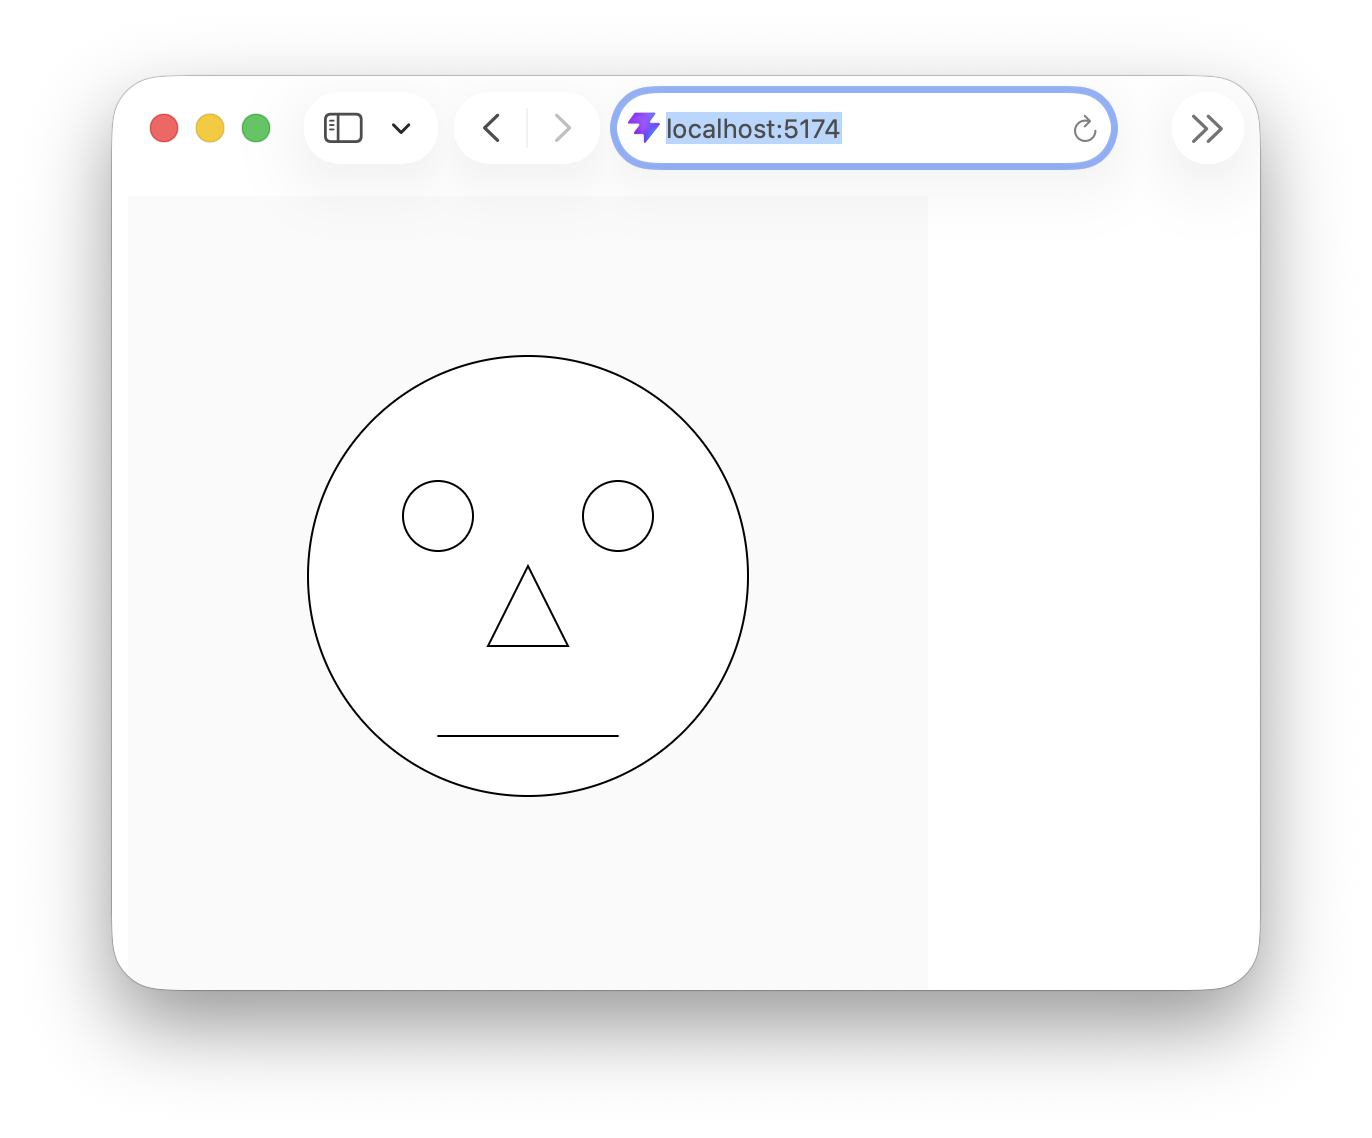
\includegraphics[width=0.6\linewidth]{figures/chapter02/simple-face.png}
    \caption{\ref{lst:chapter02-simple-face}の実行例}
    \label{fig:chapter02-simple-face}
\end{figure}

このサンプルでは、大きな円を顔、小さな円を目、三角形を鼻、線を口として使っています。図形を組み合わせるときには、まず大きな部品を描き、その後に細かい部品を重ねると考えやすくなります。

\begin{notebox}{circleについて}
\texttt{p.circle(x, y, d)}の3つ目の値は、半径ではなく直径です。たとえば、半径40の円を描きたいときは、3つ目に\texttt{80}を指定します。
\end{notebox}

\section{よくある間違い}

図形を描くプログラムでは、文法の間違いだけでなく、座標や数値の意味を取り違えることでも思った通りに表示されなくなります。

\begin{mistakebox}{y座標の向きを数学と同じだと思ってしまう}
p5.jsでは、下に進むほど$y$の値が大きくなります。上に動かしたいときは$y$を小さくし、下に動かしたいときは$y$を大きくします。
\end{mistakebox}

\begin{mistakebox}{rectの最初の2つの数値を中心だと思ってしまう}
\texttt{rect}の最初の2つの数値は、基本的に左上の座標です。\texttt{ellipse}や\texttt{circle}の中心座標とは意味が違います。
\end{mistakebox}

\begin{mistakebox}{p.を付け忘れる}
instance modeでは、\texttt{circle(...)}ではなく\texttt{p.circle(...)}のように書きます。p5.jsの命令を使うときは、前に\texttt{p.}を付けることを確認しましょう。
\end{mistakebox}

\begin{mistakebox}{描く順番を意識していない}
後から描いた図形は前に描いた図形の上に重なります。図形が隠れてしまったときは、命令の順番を見直しましょう。
\end{mistakebox}

\section{まとめ}

この章では、p5.jsで基本的な図形を描く方法を学びました。キャンバスは\texttt{p.createCanvas}で作り、点、線、円、楕円、長方形、三角形、四角形をそれぞれ専用の命令で描きます。

また、p5.jsの座標では左上が原点で、下に進むほど$y$の値が大きくなることを確認しました。さらに、図形は命令の順番通りに描かれ、後から描いた図形が手前に見えることも学びました。

\section{演習問題}

この章の演習では、座標と基本図形の描き方を確認します。最初はサンプルの数値を少し変えるところから始め、最後は複数の図形を組み合わせて自分の絵を作ってみましょう。

\begin{pointbox}{関数名と実際のコードの書き方}
本書では、関数の名前そのものを説明するときは、\texttt{point}関数や\texttt{line}関数のように書きます。
一方、TypeScript + p5.js instance modeのプログラムとして書くときは、\texttt{p.point(...)}や\texttt{p.line(...)}のように、前に\texttt{p.}を付けます。
演習で\texttt{point}関数と書かれている場合も、実際のコードでは\texttt{p.point(...)}の形で書いてください。
\end{pointbox}

\begin{enumerate}
    \item \texttt{p.createCanvas(400, 300)}の数値を変えて、横長のキャンバスと縦長のキャンバスを作ってください。
    \item \texttt{point}関数を3回以上使い、キャンバスの別々の場所に点を描いてください。
    \item \texttt{line}関数を使い、左上から右下へ向かう線と、左下から右上へ向かう線を描いてください。
    \item \texttt{circle}関数の直径を変えて、大きい円と小さい円を描いてください。
    \item \texttt{ellipse}関数を使い、横長の楕円と縦長の楕円を描いてください。
    \item \texttt{rect}関数を使い、同じ大きさの長方形を3つ、別々の位置に描いてください。
    \item \texttt{triangle}関数の頂点の数値を変えて、細長い三角形を作ってください。
    \item サンプルプログラム~\ref{lst:chapter02-drawing-order}で、描画順を入れ替えて、円が長方形の上に見える場合と、長方形が円の上に見える場合を比べてください。
    \item 円、三角形、線を組み合わせて、顔以外の簡単な絵を作ってください。
    \item 挑戦問題として、家、ロボット、乗り物など、複数の図形を組み合わせた作品を1つ作ってください。
\end{enumerate}
